\section{Princípios de Avaliação da Segurança Web}

\subsection{Tipos de Testes de Penetração}

A avaliação da segurança em aplicações web recorre, frequentemente, a testes de penetração (\textit{pentesting}). Estes testes consistem na simulação controlada de ataques informáticos, com o objetivo de identificar vulnerabilidades que possam ser exploradas por atacantes. É uma prática fundamental em cibersegurança, pois permite analisar a capacidade de resistência de uma aplicação perante ameaças reais, sem comprometer o seu funcionamento.

Consoante o grau de acesso à aplicação, os testes de penetração podem ser classificados em três modelos principais:

\begin{flushleft}
\textbullet\ \textbf{Testes de Caixa-Preta (\textit{Black-box}):} Aqui o avaliador não tem qualquer informação interna sobre a aplicação, aproximando-se da perspetiva de um atacante externo. A análise é feita exclusivamente através da interação com a aplicação em execução, sem qualquer acesso ao código-fonte ou à documentação da arquitetura.

\vspace{0.4cm}

\textbullet\ \textbf{Testes de Caixa-Branca (\textit{White-box}):} Neste caso, o avaliador tem acesso total a todos os elementos do sistema, incluindo o código-fonte, bases de dados e configurações dos servidores. Permite uma análise exaustiva e é especialmente útil na deteção de falhas lógicas ou estruturais.

\vspace{0.4cm}

\textbullet\ \textbf{Testes de Caixa-Cinzenta (\textit{Grey-box}):} Este modelo híbrido trata-se de uma abordagem intermédia, em que o avaliador tem acesso parcial ao sistema. Por exemplo, poderá ter acesso ao código do \textit{frontend} ou a credenciais de utilizadores com permissões limitadas. A abordagem caixa-cinzenta representa um equilíbrio entre o realismo da caixa-preta e a profundidade da caixa-branca, sendo frequentemente considerada a mais eficiente em termos de custo-benefício em diversos cenários de teste.
\end{flushleft}

Estas abordagens são amplamente reconhecidas nas boas práticas de engenharia de software e de testes de segurança \cite{ref37}.

\subsection{Justificação da Abordagem Adotada: Caixa-Cinzenta (\textit{Grey-box})}

No âmbito deste projeto, a abordagem de caixa-cinzenta foi considerada a mais adequada, tendo em conta as restrições impostas pela plataforma Base44. Sendo uma solução \textit{no-code}, baseada em inteligência artificial, o acesso ao \textit{backend} e à configuração do servidor está bloqueado. No entanto, todo o código do lado do cliente (\textit{HTML}, \textit{CSS} e \textit{JavaScript}) está disponível, o que permite realizar uma análise focada no \textit{frontend}.

A imagem seguinte ajuda a visualizar, de forma esquemática, a abordagem adotada neste projeto.

\begin{figure}
    \centering
    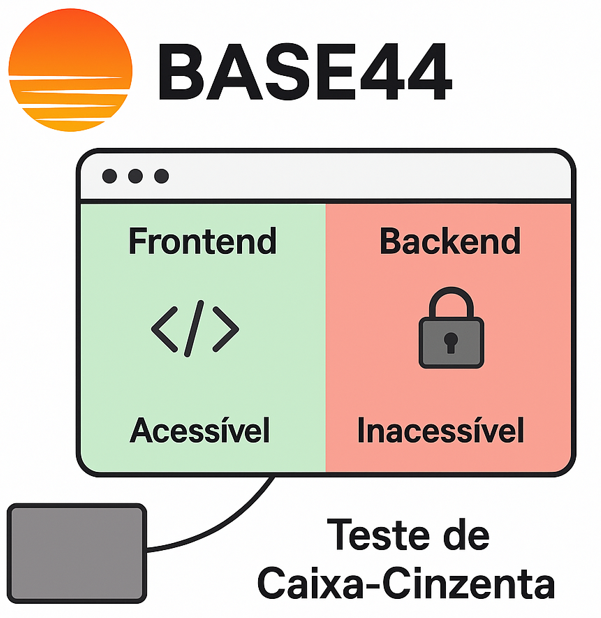
\includegraphics[width=0.4\linewidth]{imagens/diagrama.png}
    \caption{Representação esquemática da abordagem de caixa-cinzenta aplicada à Base44.}
    \label{fig:modelo_base44}
\end{figure}

Tal como representado na Figura~\ref{fig:modelo_base44}, apenas o \textit{frontend} da aplicação se encontra acessível para análise, enquanto o \textit{backend} permanece inacessível. Esta separação entre as duas camadas reflete as limitações impostas pela Base44 e ilustra bem a natureza da abordagem de caixa-cinzenta.

O diagrama reforça que, apesar do acesso restrito à infraestrutura do servidor, é possível aplicar técnicas de análise sobre os recursos disponíveis no lado do cliente. Esta abordagem equilibrada permite avaliar potenciais riscos de segurança de forma ética, segura e adequada ao contexto de plataformas \textit{no-code}.

A secção seguinte irá detalhar as ferramentas selecionadas, bem como a justificação técnica da sua utilização no âmbito do projeto.


\subsection{Métodos de Testes, Ferramentas Comuns e Abordagem Escolhida}

\subsubsection{Ferramentas automatizadas}

\paragraph{sqlmap}

é uma ferramenta automatizada
destinada à deteção e exploração de vulnerabilidades de injeção SQL em aplicações web.
Permite identificar parâmetros vulneráveis, avaliar técnicas de injeção
e, quando autorizado e possível, extrair dados a partir da base de dados alvo \cite{ref2}.
sqlmap é útil para demonstrar vetores de ataque e validar hipóteses de vulnerabilidade
em ambientes controlados; contudo, a sua utilização em sistemas de produção exige autorização explícita,
dado o elevado risco de impacto sobre a disponibilidade e confidencialidade dos dados \cite{ref3}.

\paragraph{nmap}
(Network Mapper) é uma ferramenta de mapeamento e descoberta de redes,
utilizada para identificar hosts ativos, portas abertas, serviços em execução e possíveis versões de software.
Fornece funcionalidades de reconhecimento essenciais nas fases iniciais de um teste de segurança \cite{ref1},
permitindo construir um inventário de superfície de ataque e orientar avaliações subsequentes.
nmap pode ser utilizado para ilustrar práticas de reconhecimento e perfilagem de rede,
mas deve ser usado com parcimónia e sempre dentro do âmbito autorizado,
pois varrimentos agressivos podem ser interpretados como atividade intrusiva.

\paragraph{nikto}

é um \textit{scanner} de servidores web orientado para a identificação de configurações incorretas,
ficheiros e \textit{endpoints} públicos potencialmente perigosos,
e componentes desatualizados com vulnerabilidades conhecidas \cite{ref21}.
Embora não tenha a sofisticação de \textit{scanners} comerciais,
é valioso para detetar rapidamente questões de configuração e itens de segurança negligenciados
que podem ser explorados em conjunção com outras falhas.
Para fins de investigação académica, nikto permite demonstrar vulnerabilidades de superfície web
e e problemas de \textit{hardening}, mantendo-se, tal como as outras ferramentas,
sujeito a restrições éticas e legais quando aplicado a sistemas
que não pertençam ao âmbito definido pelo estudo.

\subsubsection{Análise manual}
\paragraph{Revisão de código-fonte} — Leitura de ficheiros \textit{HTML}, \textit{JavaScript} e de configuração
para identificar segredos expostos \cite{ref12}, padrões inseguros ou lógica vulnerável no lado do cliente.
\paragraph{Ferramentas de programador do navegador} — Utilizadas para inspecionar o DOM,
pedidos de rede, \textit{cookies}, armazenamento local (\textit{localStorage}/\textit{sessionStorage})
e a execução de \textit{JavaScript}, permitindo observar o comportamento em tempo real
e potenciais falhas no \textit{frontend} \cite{ref1}.

\subsubsection{Testes estáticos vs. dinâmicos}
\paragraph{Testes estáticos} analisam o código e artefactos sem os executar
(por exemplo, revisão de \textit{JS}/\textit{HTML}, pesquisa de segredos, análise de mapas de origem \cite{ref20}).
São de baixo impacto e adequados quando apenas estão disponíveis recursos do lado do cliente.
\paragraph{Testes dinâmicos} envolvem interação direta com sistemas em execução
(por exemplo, injeção de \textit{payloads}, \textit{fuzzing} de \textit{endpoints}, exploração de lógica no servidor).
Embora possam identificar vulnerabilidades em tempo real,
implicam maior risco e requerem autorização explícita \cite{ref4}.

\subsection{Justificação da Abordagem Escolhida}
Tendo em conta que o presente estudo incide sobre aplicações exportadas da plataforma Base44 \cite{ref16},
o acesso disponível limita-se aos componentes do \textit{frontend}.
Por este motivo, a abordagem escolhida foca-se na análise estática de baixo impacto,
complementada com sondagens manuais seguras,
garantindo que todas as atividades são realizadas de forma ética e sem afetar
a integridade do ambiente de alojamento.

Será utilizada a combinação de ferramentas e técnicas seguintes:
as \textit{DevTools} do navegador para inspeção de \textit{localStorage},
\textit{service workers} \cite{ref8} e \textit{cache};
\textit{Burp Suite} ou \textit{OWASP ZAP} \cite{ref23} para varrimento controlado
de vulnerabilidades e verificação das evidências;
\textit{DOMPurify} em conjunto com a aplicação de cabeçalhos CSP \cite{ref25}
para mitigação de XSS;
e um \textit{nginx} auto-alojado para forçar \textit{TLS 1.3}
e configurar cabeçalhos de segurança \cite{ref19} no nível do servidor.

Ferramentas e técnicas que requerem interações com o \textit{backend},
como \textit{sqlmap} (injeção \textit{SQL}), \textit{nikto} (\textit{scanner web} dinâmico)
ou \textit{nmap} (varrimentos de rede), foram consideradas, mas não serão utilizadas,
pois excedem o escopo do projeto e não são compatíveis com a política de ética e segurança definida.

Assim sendo, a abordagem selecionada permite avaliar de forma responsável e ética
a superfície de ataque do \textit{frontend} das aplicações Base44,
identificar vulnerabilidades relevantes e aplicar correções demonstráveis,
enquanto se minimiza o risco de impacto sobre o ambiente de alojamento
ou os dados dos utilizadores \cite{ref27}.
Esta escolha garante que os objetivos do projeto — "reproduzir, corrigir e documentar
vulnerabilidades de forma segura e eficaz” — podem ser atingidos
dentro do período de execução previsto.

\newpage